\chapter{Well Representation}
\label{chapter-well-representation}

This chapter shows how the well has been modeled in the simulator developed in this project.
%
According to \cite{Ertekin2001}, wells are considered to be internal boundaries of the reservoir system, and therefore boundary conditions must be specified for the problem to be solved.
%
One possible boundary condition is to utilize a specified flowing sandface pressure $p_{wf}$, characterizing a Dirichlet-type boundary condition.
%
Another approach is by specifying a well flow rate, which characterizes a Neumann-type boundary condition.
%
This simulator has been developed considering the well to be flow-rate specified.
%
The well will be linked to the single-phase flow equation, Eq. \ref{equation-single-phase-flow-discretized-rearranged}, by the utilization of a source/sink term $q_{sc}$.
%
This term is present in every cell of the model, but it is only non-zero if the grid block contains a producing or injecting well completion.
%
The source/sink term $q_{sc}$ can change with time, enabling the flow rate to be changed in the simulation input.
%
Figure \ref{figure-well-flow-rate-example} shows an example of $q_{sc}$ for a flow-rate specified well.
%
The values of $q_{sc}$ are negative in this graphic since the well is set to be producing, and negative values stand for production, while positive ones represent injection.
%
\begin{figure}[h]
	\centering
	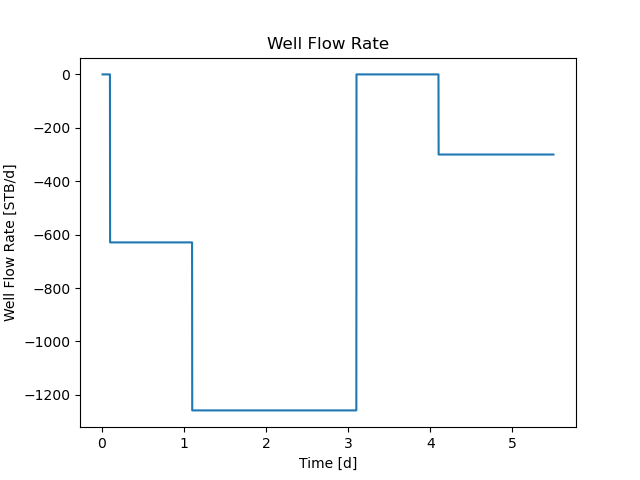
\includegraphics[width=0.7\textwidth]{figure-well-flow-rate-example.png}\\
	\caption{Example of a flow-rate specified well.}
	\label{figure-well-flow-rate-example}
\end{figure}
%
Considering a steady-state flow near the wellbore, the radial form of Darcy's law is:
%
\begin{equation}
	q=\frac{-2\pi \beta_c k h r_w}{\mu}\frac{\partial p}{\partial r}\Bigg|_{r=r_w},
\end{equation}
%
in which $r_w$ is the well radius.
%
Rearranging and considering a flow rate fixed in a specific value:
%
\nomenclature[R]{$r_w$}{Well radius}
\nomenclature[R]{$r$}{Radial dimension for cilindrical coordinates}
\nomenclature[R]{$h$}{Reservoir height}
\nomenclature[R]{$c$}{Generic constant}
%
\begin{equation}
	\frac{\partial p}{\partial r}\Bigg|_{r=r_w}=-\frac{\mu}{2\pi\beta_c khr_w}q_{sp}.
\end{equation}
%
Since $\mu$, $\beta_c$, $k$, $h$ and $r_w$ are specific for the problem, the pressure gradient should be constant:
%
\begin{equation}
	\frac{\partial p}{\partial r}=c,
\end{equation}
%
in which $c$ represents a generic constant.
%
Thus, it characterizes a Neumann-type boundary condition.
%
Determining the well performance in a given perforated grid block requires knowing the grid block pressure, $p_{i,j,k}$, the flowing sandface pressure, $p_{wf}$, and the production rate, $q_{sc}$.
%
Therefore, it is necessary to develop equations to relate the grid block unknowns to the unknowns added by the well model.

\section{Inflow Performance Relationship}

For a steady-state flow in the wellbore's vicinity, the radial form of Darcy's law is:
%
\begin{equation}
	q=-\frac{2\pi\beta_c k_H h r}{\mu} \frac{\partial p}{\partial r},
\end{equation}
%
in which $k_H$ is the radial permeability, equals to the geometrical mean of $k_x$ and $k_y$.
%
Rearranging and integrating it:
%
\begin{equation}
	\int_{r_w}^{r}\frac{1}{r}\partial r = -\frac{2\pi\beta_c k_H h}{q \mu}\int_{p_{wf}}^{p}\partial p.
\end{equation}
%
Thus:
%
\nomenclature[R]{$p_{wf}$}{Bottom-hole flowing pressure}
\nomenclature[R]{$k_H$}{Radial permeability}
%
\begin{equation}
	\label{equation-darcys-law-rearranged-for-a-well}
	p=p_{wf}-\frac{q \mu}{2 \pi \beta_c k_H h}\ln\left(\frac{r}{r_w}\right).
\end{equation}
%
In terms of flow rate:
%
\nomenclature[R]{$p_e$}{Reservoir external pressure}
\nomenclature[R]{$r_e$}{Reservoir external radius}
%
\begin{equation}
	q=-\frac{2\pi\beta_c k_H h}{\mu \log_e(r_e/r_w)} (p_e - p_{wf}),
\end{equation}
%
where $p_e$ is the reservoir external pressure, and $r_e$ is the reservoir external radius. Considering the flow rate in the surface conditions:
%
\begin{equation}
	q_{sc}=-\frac{2\pi\beta_c k_H h}{\mu B \ln(r_e/r_w)} (p_e - p_{wf}),
\end{equation}
%
This is the inflow performance relationship (IPR) for an undamaged well under a steady-state flow.
%
However, in reservoir engineering, the IPR is usually expressed in terms of the average reservoir pressure, instead of the external boundary pressure.
%
According to \cite{Ertekin2001}, for a cylindrical reservoir, its average pressure, $\bar{p}$, could be described as:
%
\begin{equation}
	\label{equation-average-pressure-of-a-cylindrical-reservoir}
	\bar{p}=\left[ \int_{r_w}^{r_e} 2 \pi r h p dr \right]/\left[ \int_{r_w}^{r_e} 2 \pi r h dr \right].
\end{equation}
%
Substituting Eq. \ref{equation-darcys-law-rearranged-for-a-well} in Eq. \ref{equation-average-pressure-of-a-cylindrical-reservoir}:
%
\begin{equation}
	\bar{p}=\frac{2}{(r_e^2-r_w^2)} \int_{r_w}^{r_e} p r dr.
\end{equation}
%
Developing the equation:
%
\begin{equation}
	\bar{p}=\frac{2}{(r_e^2-r_w^2)} \int_{r_w}^{r_e} \left[ p_{wf} - \frac{q \mu}{2 \pi \beta_c k_H h} \log_e \left(\frac{r_e}{r_w}\right) \right] r dr.
\end{equation}
%
Solving the integral in the right term:
%
\begin{equation}
	\bar{p}= p_{wf} - \frac{q \mu}{2 \pi \beta_c k_H h (r_e^2-r_w^2)} \left[ r_e^2 \log_e \left(\frac{r_e}{r_w}\right) (r_e^2-r_w^2) \right].
\end{equation}
%
When $r_e >> r_w$, the term $(r_e^2-r_w^2)$ tends to $r_e^2$. 
%
Rearranging:
%
\begin{equation}
	\bar{p}=p_{wf} - \frac{q \mu}{2 \pi \beta_c k_H h}\left[ \log_e \left(\frac{r_e}{r_w}\right)\right]
\end{equation}
%
In terms of flow rate:
%
\begin{equation}
	q = \frac{- 2 \pi \beta_c k_H h}{\mu \left[ \log_e \left(\frac{r_e}{r_w}\right)\right]} (\bar{p}-p_{wf}),
\end{equation}
%
In standard conditions:
%
\begin{equation}
	q_{sc} = \frac{- 2 \pi \beta_c k_H h}{\mu B \left[ \log_e \left(\frac{r_e}{r_w}\right)\right]} (\bar{p}-p_{wf}),
\end{equation}
%
The skin factor $s$ is a dimensionless pressure drop utilized for representing damage (if positive) or a stimulation (if negative) in the wellbore.
%
Including it in the equation:
%
\begin{equation}
	\label{equation-inflow-performance-relationship}
	q_{sc} = \frac{- 2 \pi \beta_c k_H h}{\mu B \left[ \log_e \left(\frac{r_e}{r_w}\right) + s\right]} (\bar{p}-p_{wf}),
\end{equation}
%
This is the final form of the IPR equation for a well considering a steady-state flow in its boundaries.
%
Utilizing the definition of the well's productivity index (PI), $J_w$:
%
\begin{equation}
	\label{equation-productivity-index}
	J_w = \frac{ 2 \pi \beta_c k_H h}{\mu B\left[ \log_e \left(\frac{r_e}{r_w}\right) + s\right]},
\end{equation}
%
\nomenclature[R]{$J_w$}{Productivity index for the well}
\nomenclature[A]{PI}{Productivity Index}
\nomenclature[A]{IPR}{Inflow Performance Relationship}
%
thus, the IPR equation could be simplified as:
%
\begin{equation}
	q_{sc} = - J_w \left( \bar{p}-p_{wf} \right),
\end{equation}
%
The next subchapter shows a model for calculating $r_e$ as the equivalent well radius $r_{eq}$.
%
Assembling that definition into Eq. \ref{equation-productivity-index} will make it possible to calculate $q_{sc}$ and utilize it as the sources/sinks terms in the single-phase flow equation, \ref{equation-single-phase-flow-discretized-rearranged}.
%
However, this is only possible in rate-specified wells passing across a single perforated grid block.
%
In wells with multiple perforated layers, it is necessary to decompose the total specified well flow rate into individual flow rates of each perforated grid block.
%
This process will be shown in the last part of this chapter.

\section{Peaceman Model}

The simulator has been developed for considering a vertical well passing across the center of the grid blocks.
%
The well grid block is not necessarily square, and the simulator considers an anisotropic reservoir in terms of petrophysical proprieties.
%
Then, the $r_e$ in the Eq. \ref{equation-productivity-index} will be approximated by the equivalent well radius $r_{eq}$ in the Peaceman model for non-square grid blocks with anisotropic permeability.
%
\begin{figure}[h]
	\centering
	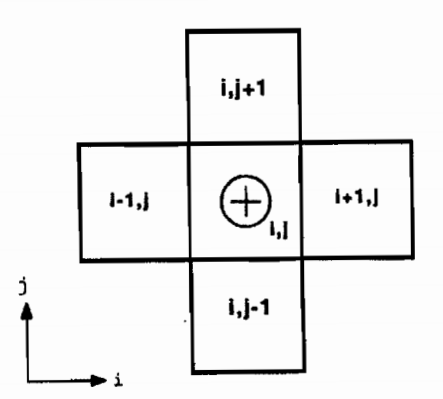
\includegraphics[width=0.5\linewidth]{figure-well-vertical-section.png}
	\caption{Vertical section of the wellbore and the grid blocks considered in its flow model. Source: \cite{Ertekin2001}.}
	\label{figure-well-vertical-section}
\end{figure}
%
According to \cite{Ertekin2001}, the equivalent well radius, $r_{eq}$, in which the steady-state reservoir pressure is equal to the pressure in the well grid block, $p_{i,j,k}$, is:
%
\begin{equation}
	\label{equation-equivalent-well-radius-peaceman}
	r_{eq} = 0.28 \frac{ \left\lbrace \left[ (k_y/k_x)^{\sfrac{1}{2}} (\Delta x)^2 \right] + \left[ (k_x/k_y)^{\sfrac{1}{2}} (\Delta y)^2 \right]\right\rbrace^{\sfrac{1}{2}}}{ (k_y/k_x)^{\sfrac{1}{4}} + (k_x/k_y)^{\sfrac{1}{4}}}
\end{equation}
%
This is the Peaceman model for non-square grid blocks with anisotropic permeability.
%
This definition of $r_{eq}$ can then be assembled into Eq. \ref{equation-productivity-index}, making possible the calculation of the well productivity index, $J_w$.

\section{Well Model for Multiple Perforated Layers}

The Eqs. \ref{equation-darcys-law-rearranged-for-a-well} and \ref{equation-equivalent-well-radius-peaceman} alone can only represent a well with producing/injecting intervals inside a single grid block.
%
For wells with more than one cell containing open completions, a different approach is required.
%
Figure \ref{figure-well-with-multiple-layers} illustrates a well passing across multiple layers.
%
\begin{figure}[h]
	\centering
	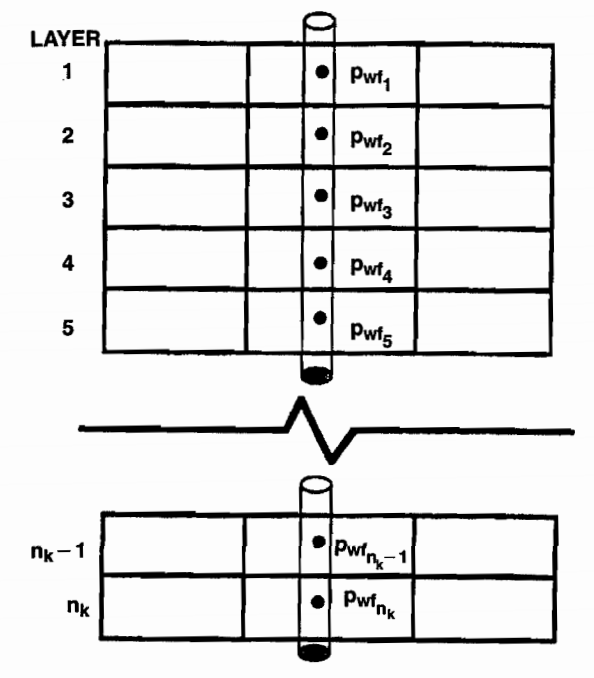
\includegraphics[width=0.7\linewidth]{figure-well-with-multiple-layers.png}
	\caption{Wellbore with multiple layers. Source: \cite{Ertekin2001}.}
	\label{figure-well-with-multiple-layers}
\end{figure}
%
Each perforated cell can and probably have different proprieties such as permeabilities, $k_{H_k}$, skin factor, $s_k$, radii, $r_{w_k}$, and, consequently, productivity indexes, $J_{w_k}$.
%
Furthermore, each perforated layer can have different flowing sandface pressures, $p_{{wf}_k}$, and grid blocks pressures, ${p_k}$.
%
In reservoir engineering, flow-rate specified wells usually are described by their total flow rate in surface conditions, $q_{spsc}$.
%
That, however, is not the flow rate value utilized in the source/sink terms $q_{sc}$ in the Eq. \ref{equation-single-phase-flow-discretized-rearranged}.
%
$q_{spsc}$ represents the flow rate of the entire well, while $q_{sc}$ is only the individual flow rate of a given grid block region.
%
Decomposing this total flow rate, $q_{spsc}$, in the individual flow rates of each layer, $q_{{sc}_k}$, can not be done by just dividing it equally for each perforated grid block.
%
Since each of the cells has different $p_{i,j,k}$, $p_{wf}$ and $J_{w}$, the $q_{{sc}_k}$ are not necessarily equal fractions of $q_{spsc}$.
%
Figures \ref{figure-well-model-unrealistic} and \ref{figure-well-model-realistic} help to visualize this idea.
%
The first image shows an unrealistic well model in which each grid block in the wellbore region has the same source/sink term, while the second image shows a realistic model, in which the total flow rate $q_{spsc}$ is decomposed in different individual flow rates $q_{{sc}_k}$ for each grid block.
%
\begin{figure}[H]
	\centering
	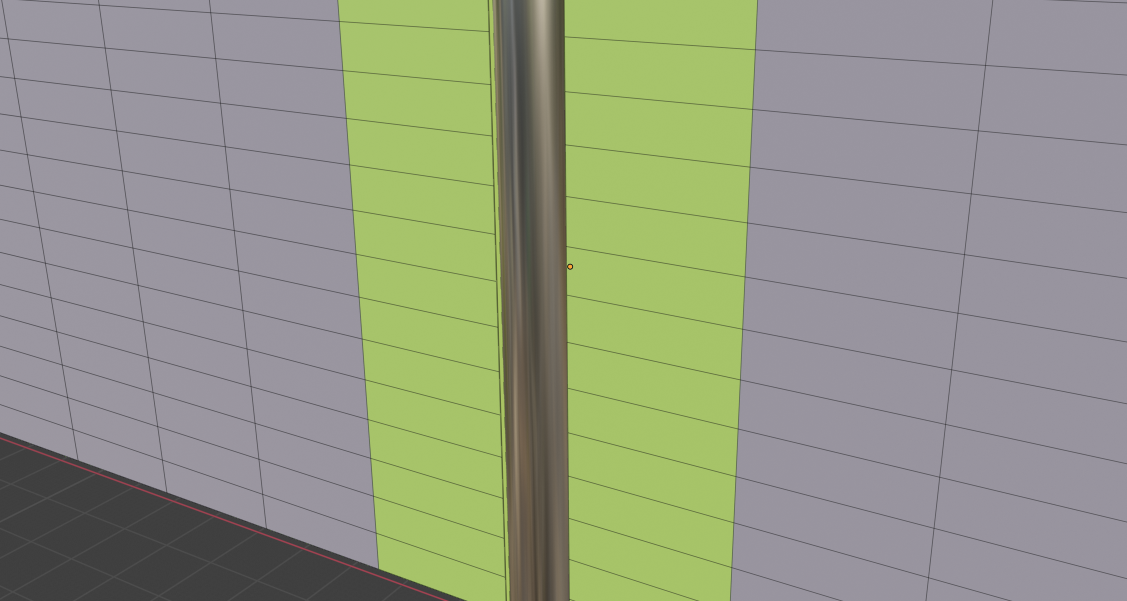
\includegraphics[width=0.8\linewidth]{figure-well-model-unrealistic.png}
	\caption{Example of well completions passing across multiple grid blocks. The color represents the source/sink term of each grid block in a given time step for a production scenario. This image represents an unrealistic scenario since each layer has the same value of individual flow rate.}
	\label{figure-well-model-unrealistic}
\end{figure}
%
\begin{figure}[h]
	\centering
	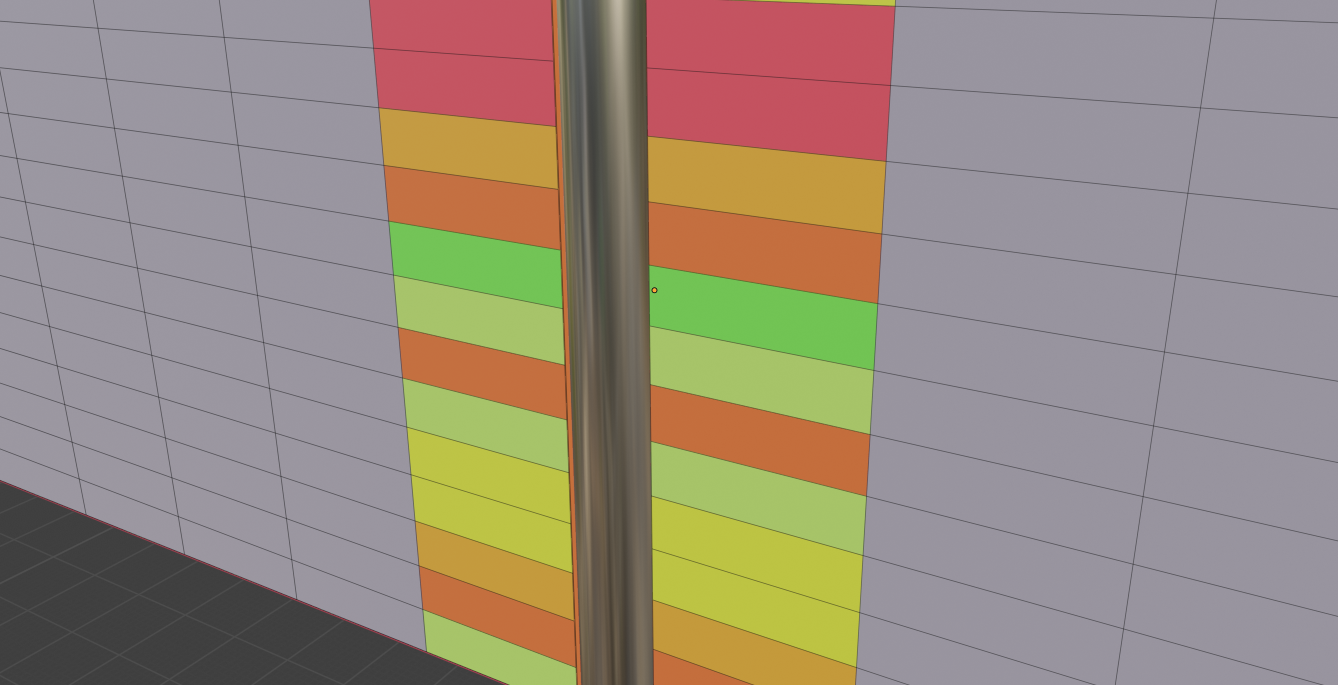
\includegraphics[width=0.8\linewidth]{figure-well-model-realistic.png}
	\caption{Example of well completions passing across multiple grid blocks. The color represents the source/sink term of each grid block in a given time step for a production scenario. This image depicts a realistic scenario in which each layer has a different value of individual flow rate.}
	\label{figure-well-model-realistic}
\end{figure}
%
The well model developed in this project approaches the multilayering by a method proposed by \cite{Ertekin2001}.
%
In a final analysis, the objective is to calculate the individual flow rates $q{sc_k}$ for all the cells in the well perforations domain.
%
Then it would be possible to input them as the source/sink terms in the single-phase flow equation, \ref{equation-single-phase-flow-discretized-rearranged}.
%
This needs to be done for each time step, since $q{sc_k}$ depends on some proprieties that can change with time (e.g. $\mu$, $B$, $\gamma_{wb}$, $\bar{p}$ and $q_{spsc}$).
%
This process will result in an iteration, since the specific weight inside the wellbore $\gamma_{wb}$ and the flowing sandface pressure $p_{wf}$ are unknowns and mutually dependent.
%
This process will be described below.

The IPR equation, Eq. \ref{equation-inflow-performance-relationship}, for a given perforated grid block in a layer $k$, is:
%
\nomenclature[R]{$s$}{Skin factor}
\nomenclature[R]{$r_{eq}$}{Equivalent radius}
%
\begin{equation}
	q_{{sc}_k} = \frac{- 2 \pi \beta_c k_{H k} h_k}{\mu_k B_k \left[ \log_e \left(\frac{r_{eq_k}}{r_w}\right) + s_k\right]} (\bar{p_k}-p_{{wf}_k}),
\end{equation}
%
which could be rewritten in terms of the PI as:
%
\begin{equation}
	\label{equation-inflow-performance-relationship-multilayer}
	q_{{sc}_k} = - J_{w_k} \left( p_k - p_{wf_k} \right),
\end{equation}
%
in which:
%
\begin{equation}
	\label{equation-productivity-index-multilayer}
	J_{w_k} = \frac{ 2 \pi \beta_c k_{H_k} h_k}{\mu_k B_k\left[ \log_e \left(\frac{r_{eq_k}}{r_w}\right) + s_k\right]}.
\end{equation}
%
The total flow rate of the well, $q_{spsc}$, is the sum of all the individual flow rates of the perforated layers, $q_{{sc}_k}$. Thus:
%
\begin{equation}
	q_{spsc} = - \sum_{k} J_{w_k} (p_k- p_{wf_k}),
\end{equation}
%
in which $k \in \psi_w$, where $\psi_w$ is the set of all the perforated grid blocks.
%
Similarly to the variables in the flow equation, it is necessary to determine a time level in which the well flow rates will be evaluated.
%
The simple iteration method has been utilized, where the IPR parameters are evaluated at the time level $n+1$, but at the previous iteration level, $\nu$.

For determining the pressure distribution inside the wellbore, the conventional approach in reservoir simulation is to neglect the friction losses inside the tubing and downhole equipment.
%
Although this is not the most realistic approach, integrating those effects in a reservoir simulator would result in a system with high complexity, requiring an unfeasible amount of computational power.
%
There are simulators specially made for analyzing the flow inside the well and pipeline systems, but those are not commonly integrated to reservoir simulators.
%
After neglecting the friction losses inside the wellbore, the flowing sandface pressures for each layer, $p_{wf_k}$, can be obtained by:
%
\nomenclature[U]{$ref$}{Reference}
\nomenclature[U]{$k$}{Layer index}
\nomenclature[G]{$\gamma_{wb}$}{Average specific weight inside the wellbore}
\nomenclature[R]{$q_{spsc}$}{Total specified flow rate for the well in the standard conditions}
%
\begin{equation}
	p_{wf_k} = p_{wf_{ref}} + \int_{H_{ref}}^{H_k} \gamma_{wb} dH,
\end{equation}
%
where $p_{wf_{ref}}$ is the flowing sandface pressure of a reference layer, and $\gamma_{wb}$ is the specific weight inside the wellbore in the perforated grid blocks.
%
For the simulator developed in this project, the selected reference layer has been the topmost perforated grid block.
%
\cite{Ertekin2001} recommends the following approximation to this integral:
%
\begin{equation}
	\label{equation-bottom-hole-pressure-multilayer}
	p_{wf_k} = p_{wf_{ref}} + \bar{\gamma}_{wb} (H_k - H_{ref}).
\end{equation}
%
in which $H_{ref}$ is the depth of the reference layer, $H_k$ is the depth of a given layer $k$ and $\gamma_{wb}$ is the average specific weight in the well for the perforated region.
%
The average flowing sandface pressure, $\bar{p}_{wf}$, could be described as the arithmetic average between the lowest and the highest pressures inside the perforated regions of the wellbore, those are $p_{{wf}_{ref}}$ and $p_{{wf}_n}$:
%
\begin{equation}
	\label{equation-average-bottom-hole-pressure-multilayer}
	\bar{p}_{wf} = \frac{p_{wf_{ref}} + p_{wf_{n}}}{2},
\end{equation}
%
where $n$ is the index of the lowermost perforated cell.
%
For allocating the quotes of the total well flow rate in each perforated layer, the following relationship is valid:
%
\begin{equation}
	q_{sc_k} = \frac{q_{sc_k}}{q_{spsc}}q_{spsc},
\end{equation}
%
Applying the IPR equation, Eq \ref{equation-inflow-performance-relationship-multilayer}:
%
\begin{equation}
	\label{equation-well-flow-rate}
	q_{sc_k} = \frac{J_{w_k} (p_k- p_{wf_k})}{\sum_{m}J_{w_m} (p_m- p_{wf_m})} q_{spsc},
\end{equation}
where $m$ and $k \in \psi_w$.
%
\cite{Ertekin2001} describes it as the potential method for multilayering.
%
Substituting the Eq. \ref{equation-bottom-hole-pressure-multilayer} in the IPR equation for the total flow rate in the well, Eq. \ref{equation-inflow-performance-relationship-multilayer}:
%
\begin{equation}
	q_{spsc} = \sum_{k} J_{w_k} \left\lbrace p_k - \left[ p_{wf_{ref}} + \bar{\gamma}_{wb} \left( H_k - H_{ref} \right)  \right]  \right\rbrace,
\end{equation}
%
Rearranging:
%
\begin{equation}
	q_{spsc} = \sum_{k} J_{w_k} \left[  p_k - \bar{\gamma}_{wb} \left( H_k - H_{ref} \right) \right] + \sum_{k} J_{w_k} p_{wf_{ref}},
\end{equation}
%
After further rearrangements, in terms of $p_{wf_{ref}}$:
%
\begin{equation}
	\label{equation-bottom-hole-pressure-multilayer-rearranged}
	p_{wf_{ref}} = \frac{\sum_{k} \left\lbrace J_{w_k} \left[ p_k - \bar{\gamma}_{wb} (H_k - H_{ref})\right] \right\rbrace + q_{spsc}}{\sum_{k}J_{w_k}},
\end{equation}
%
Since both $\bar{\gamma}_{wb}$ and $p_{wf_{k}}$ are unknowns and mutually dependent, it is necessary to perform an iterative process.
%
Table \ref{table-multilayer-well-model-algorithm} shows the iterative approach that has been utilized:

\begin{table}[htbp]
	\centering
	\caption{Algorithm for modeling a well with multiple perforated grid blocks.}
	\begin{tabular}{r l}
		\toprule
		$1)$ & At the initial conditions, $p_{wf_{k}}$ are set to be equal to $p_k$. \\
		$2)$ & $\bar{p}_{wf}$ is calculated by utilizing the Eq. \ref{equation-average-bottom-hole-pressure-multilayer}. \\
		$3)$ & $\bar{\gamma}_{wb}$ is interpolated in the fluid table for $\bar{p}_{wf}$.\\
		$4)$ & $J_{w_k}$ is calculated for each perforated cell with Eq. \ref{equation-productivity-index-multilayer}.\\
		$5)$ & $p_{wf_{ref}}$ is obtained by the Eq. \ref{equation-bottom-hole-pressure-multilayer-rearranged}.\\
		$6)$ & $p_{wf_{k}}$ is calculated with Eq. \ref{equation-bottom-hole-pressure-multilayer} for each perforated grid block.\\
		$7)$ & $\bar{p}_{wf}$ is again calculated using the Eq. \ref{equation-average-bottom-hole-pressure-multilayer}. \\
		$8)$ & $\bar{\gamma}_{wb}^{new}$ is interpolated for the new value of $\bar{p}_{wf}$.\\
		$9)$ & If $|\bar{\gamma}_{wb}^{new} - \bar{\gamma}_{wb}| > \epsilon$, $\bar{\gamma}_{wb} = \bar{\gamma}_{wb}^{new}$ and return to $4)$. Otherwise, go to $10)$.\\
		$10)$ & Finally, $q_{{sc}_k}$ is calculated with Eq. \ref{equation-well-flow-rate} for each perforated cell.\\
		\bottomrule
	\end{tabular}
	\label{table-multilayer-well-model-algorithm}
\end{table}
%
After performing this process, the individual well flow rates $q_{sc_k}$ are finally obtained.
%
Then it is possible to utilize those values in the single-phase flow equation \ref{equation-single-phase-flow-discretized-rearranged}.
%
Note that this process has to be done for each time step, since, as shown above, $q_{sc_k}$ depends on time-dependent proprieties.

